\chapter{Development of a Web-Based Visualization Tool for the Comparison of Organism Genome Properties} \label{micromeda-client}

As discussed in Chapter XXX, Micromeda's user interface is provided by a client web application. This client's role is to provide users with a streamlined interface for visualizing patterns of property and step assignment found across organisms. This assignment data is provided to the client in the form of a user uploaded Micromeda file (Section \ref{MicromedaFiles}). After upload, these files are sent to Micromeda-Server (Chapter \ref{micromeda-server}) where they are parsed and used to provide data to the client. The client can request this data through series of web application programming interface (API) endpoints (Section \ref{endpoints}) provided by Micromeda-Server. In this chapter we will discuss the client web application, called Micromeda-Client, in detail.

\section{Visualisation Design}

One of the core uses of Genome Properties assignment data is to mine it for biologically relevant patterns. These patterns are found in the presence and absence of biochemical pathways or structural features across organisms. One of the best ways to detect such patterns is through the use of data visualisation. By visualising such data we can make many types of comparisons between organisms, pathways or steps. Some examples comparisons and their research relevance are listed below and displayed in Fig. \ref{fig:client-analysis-types}. 

\begin{itemize}
\item Looking at the assignments of a single property across organisms can be used to used for the selection of subsets of organisms which may posses a specific phenotype (Fig. \ref{fig:client-analysis-types}a). In the field of genetic engineering, such comparisons useful host and gene donor selection.
\item Comparing the assignments of multiple properties could be used for identifying patterns of property conservation across organisms in a dataset (Fig. \ref{fig:client-analysis-types}c). In microbial ecology, such comparisons could be used to identify microorganisms which fit specific ecological roles.
\item Looking at the steps assignments of a single property in a single organism could be used to evaluate the correctness of the  assignment (Fig. \ref{fig:client-analysis-types}b). For example, a property might be assigned NO or PARTIAL because it is only missing a few required step assignments but possess many others which are not required (Fig. \ref{fig:client-analysis-types}b). Being able to look at all step assignments for the property may be useful for determining why a property has been given an assignment.
\item Comparing the step assignments of single property across organisms can be used to see what pathway steps are retained across organisms that differ photogenically (Fig. \ref{fig:client-analysis-types}d). For example, if a property step is not retained in a large assortment of genomes, it may not be required for a pathway or is carried out by proteins which are non-canonical (Fig. \ref{fig:client-analysis-types}d). Such non-canonical proteins may not posses domains used by Genome Properties but may still carry out the pathway step.
\end{itemize}

\begin{figure}[!ht]
  \centering
	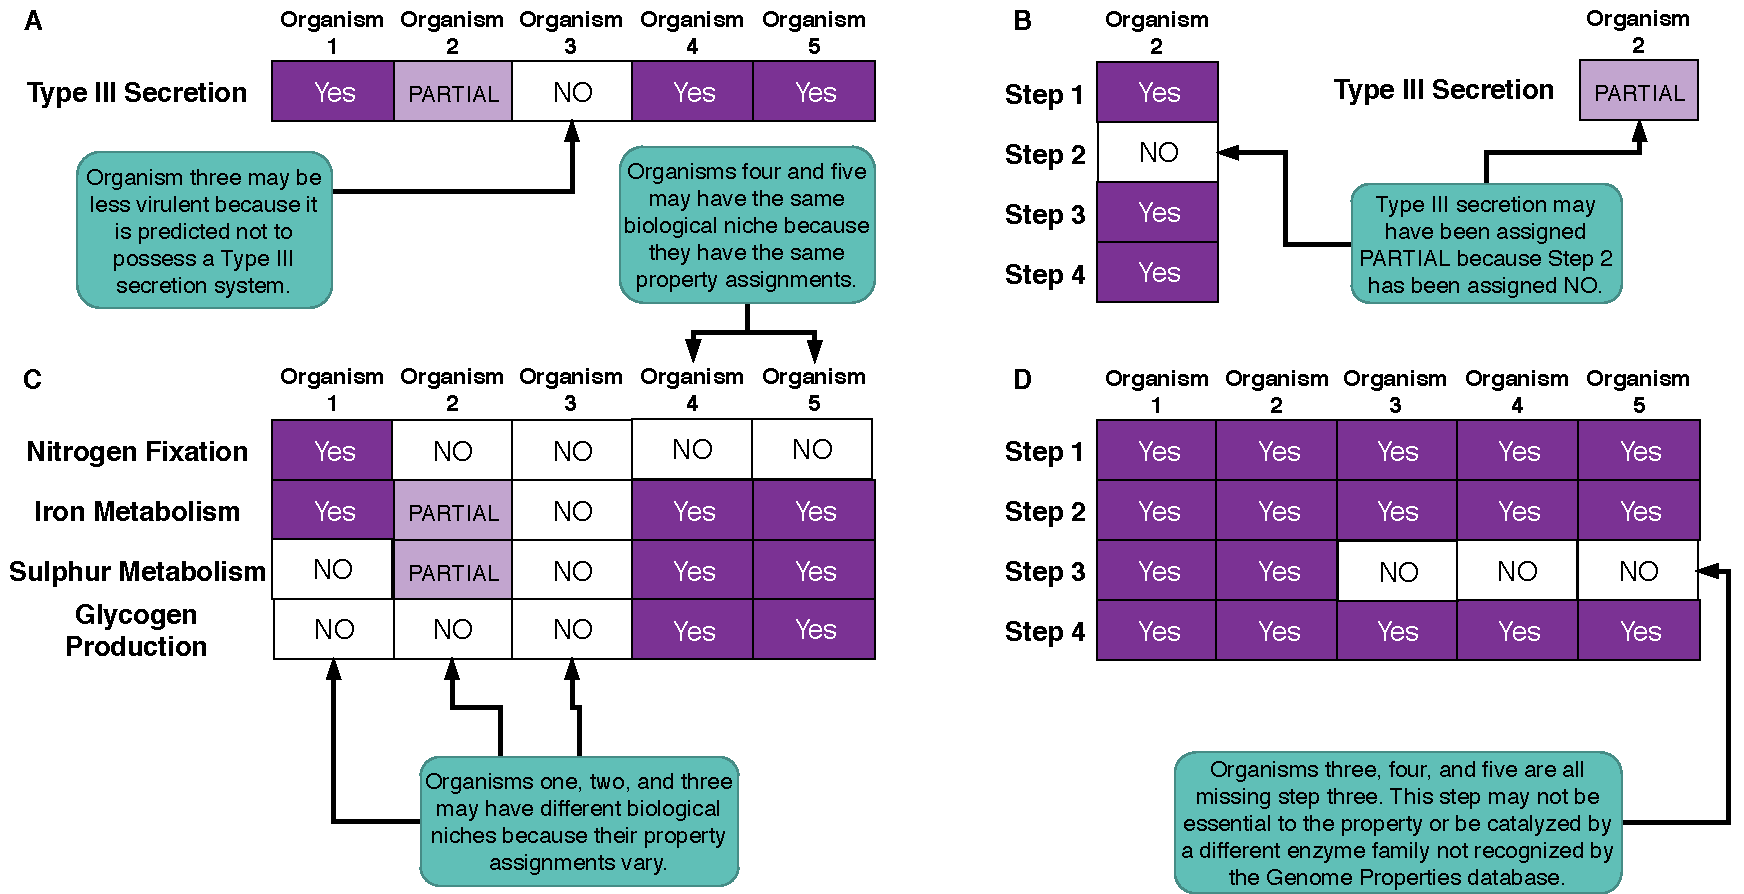
\includegraphics[width=\textwidth]{media/analysis_types.pdf}
	 \caption{Visualizations of Genome Properties data can be used to compare property and step assignments across organisms.}
	 \label{fig:client-analysis-types}
\end{figure}

If Micromeda-Client is to support the above comparison's, the data visualization method used Micromeda-Client should allow users to perform the following tasks.

\begin{itemize}
\item Track assignments across organisms.
\item Assess the magnitude of given assignments.
\item Aggregate step and property assignments into summaries.
\item Explore how these aggregate assignments are derived.
\item Quickly find assignments of interest.
\end{itemize}

When a visualization approach was select for use by Micromeda-Client, the compatibility of the visualization with these tasks was kept in mind.

\subsection{An Overview of Genome Properties Data}

Different types of data are more suitable to specific visualisation techniques and it is important to first discuss the nature of the data to be visualized before discussing why the author selected a specific visualisation type for Micromeda-Client. At its core, the data presented by Micromeda-Client consists of assignments for genome properties and their steps. Such assignments are ordinal data \cite{richardson2018genome,agresti2010analysis}, as their states of YES, PARTIAL and NO, though categorical, are ordered. Its should be noted that properties are also connected to each other in hierarchical manner \cite{richardson2018genome}. This structure can be considered hierarchical data \cite{richardson2018genome,samet1990applications}. The ordinal assignment data is also influenced by property hierarchy as the assignments of parent genome properties can be used to summarize the assignments of child genome properties or property steps \cite{richardson2018genome}. Each piece of assignment data found in a Micromeda file belongs to a specific property or step and organism. Thus, the genome property assignment data can be also considered multidimensional \cite{pedersen1999multidimensional}.

\subsection{How Assignment Data Is Visualized By Micromeda-Server}

When designing a data visualization, sometimes specific visualization techniques immediately stick out. This was the case while designing Micromeda-Client. A very apt visualization for multidimensional datasets, such as Genome Properties assignments, is a heat map \cite{wilkinson2009history,tufte2001visual}(Fig. \ref{fig:client-analysis-types}) and this is the visualization technique chosen for the client (Fig. \ref{fig:client-analysis-types}). In such a visualization, cell position is used to indicate which assignment belongs to what property or step and organism (Fig. \ref{fig:client-analysis-types}). Because most Micromeda files have less organisms than genome properties, we chose to position assignments for the same property in the same heat map row. Each assignment is from a different organisms in the dataset. This configuration leads to a heat map that is much taller than it is wide, which forces users scroll vertically. Scrolling vertically is much more convenient than horizontally as it allows the user to scroll using their mouses scroll wheel. Columns are used to group assignments from the same organism across properties and steps. The magnitude of each assignment is encoded using cell color (Fig. \ref{fig:client-analysis-types}). Since assignments are ordinal data it makes sense to encode assignments using colour saturation, rather than hue \cite{munzner2015visualization}. For Micromeda-Server the author chose to use a purple cell color scheme to insure diagram is interpretable by those with colour blindness. A web service called color brewer (\href{colorbrewer2.org}{colorbrewer2.org}) was used to select these colors and a tool called Sim Daltonism (href{github.com/michelf/sim-daltonism}{github.com/michelf/sim-daltonism}) was used to ensure the color blind compatibility of the entire diagram. A heat map was chosen over competing visualization techniques such as bubble charts \cite{tufte2001visual}, circular maps \cite{ward2002taxonomy,stothard2004circular} or tree maps \cite{shneiderman1998tree} due to the number of variables that needed to be plotted and the superior space utilization of heat maps. Heat maps have superior space utilisation as compared to circular plots because they mimic the square dimensions of the computer monitors they are displayed on (Fig. \ref{fig:circle-square}).

\begin{figure}[!ht]
  \centering
	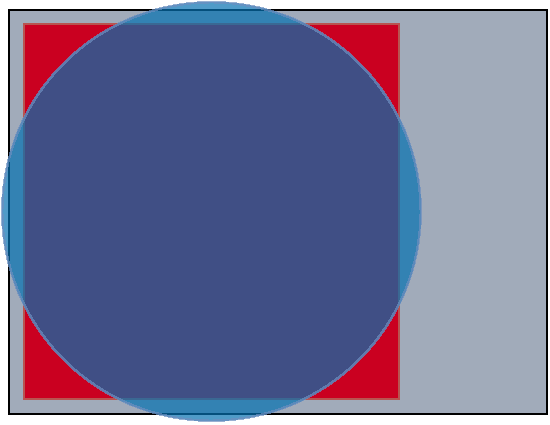
\includegraphics[width=0.7\textwidth]{media/square_vs_circle.pdf}
	 \caption{A square shape (red), as posses by a heat map, provides better space utilization on a conventional display (grey). The circle (blue) and square have the same area. A circle requires greater X and Y-axis dimensions to display the same amount of data and produces dead space at the displays corners where data cannot be presented.}
	 \label{fig:circle-square}
\end{figure}

Any visualization technique used by Micromeda-Client is also challenged by the shear size of the data to be presented. For example, if all assignments for only a few organisms were displayed in the heat map described above, then its shear size would prevent users to quickly finding assignments or tracking assignments across organisms. As of version 2.0 of the Genome Properties database, there are 1296 properties and 6525 steps. If a single heat map was generated for all properties, with each cell being 5 mm tall, such a heat map would be approximately 6.5 meters tall (i.e., fifteen vertical pages on a 24" monitor). If the same heat map was made for all property steps, the resulting heat map would be over 32.6 meters tall (i.e., seventy-five vertical pages on a 24" monitor). If both of these heat maps were combined, it would be even larger. To address this length issue, Micromeda-Client's visualization interface uses interactive aggregation and de-aggregation of assignment rows to reduce the overall length of its assignment heat map (Fig. \ref{fig:visualization-philosophy}). This reduced length facilitates rapid visual exploration of property and step assignments.

Micromeda-Client's user interface allows users to manipulate the contents of its assignment heat map to show and hide properties and steps according to their position in the Genome Properties Directed Acyclic Graph (DAG) (Fig. \ref{fig:visualization-philosophy}). Because individual properties are arranged hierarchically, the assignments of properties closer to the root of the Genome Properties DAG can be used to summarize the assignments of properties closer to its leafs (Fig. \ref{fig:visualization-philosophy}). In the context of a heat map, this means that a row of assignments for a parent property can be used to summarize the rows of assignments of its child properties. In addition, an assignment heat map row for a leaf genome property can be used to summarize the assignment rows of its steps (Fig. \ref{fig:visualization-philosophy} and Fig. \ref{fig:client-analysis-types}). Micromeda-Client provides mechanisms to expand and collapse heat map rows to display either parent summary assignments or more detailed child assignments (Fig. \ref{fig:visualization-philosophy}).

\begin{figure}[!ht]
  \centering
	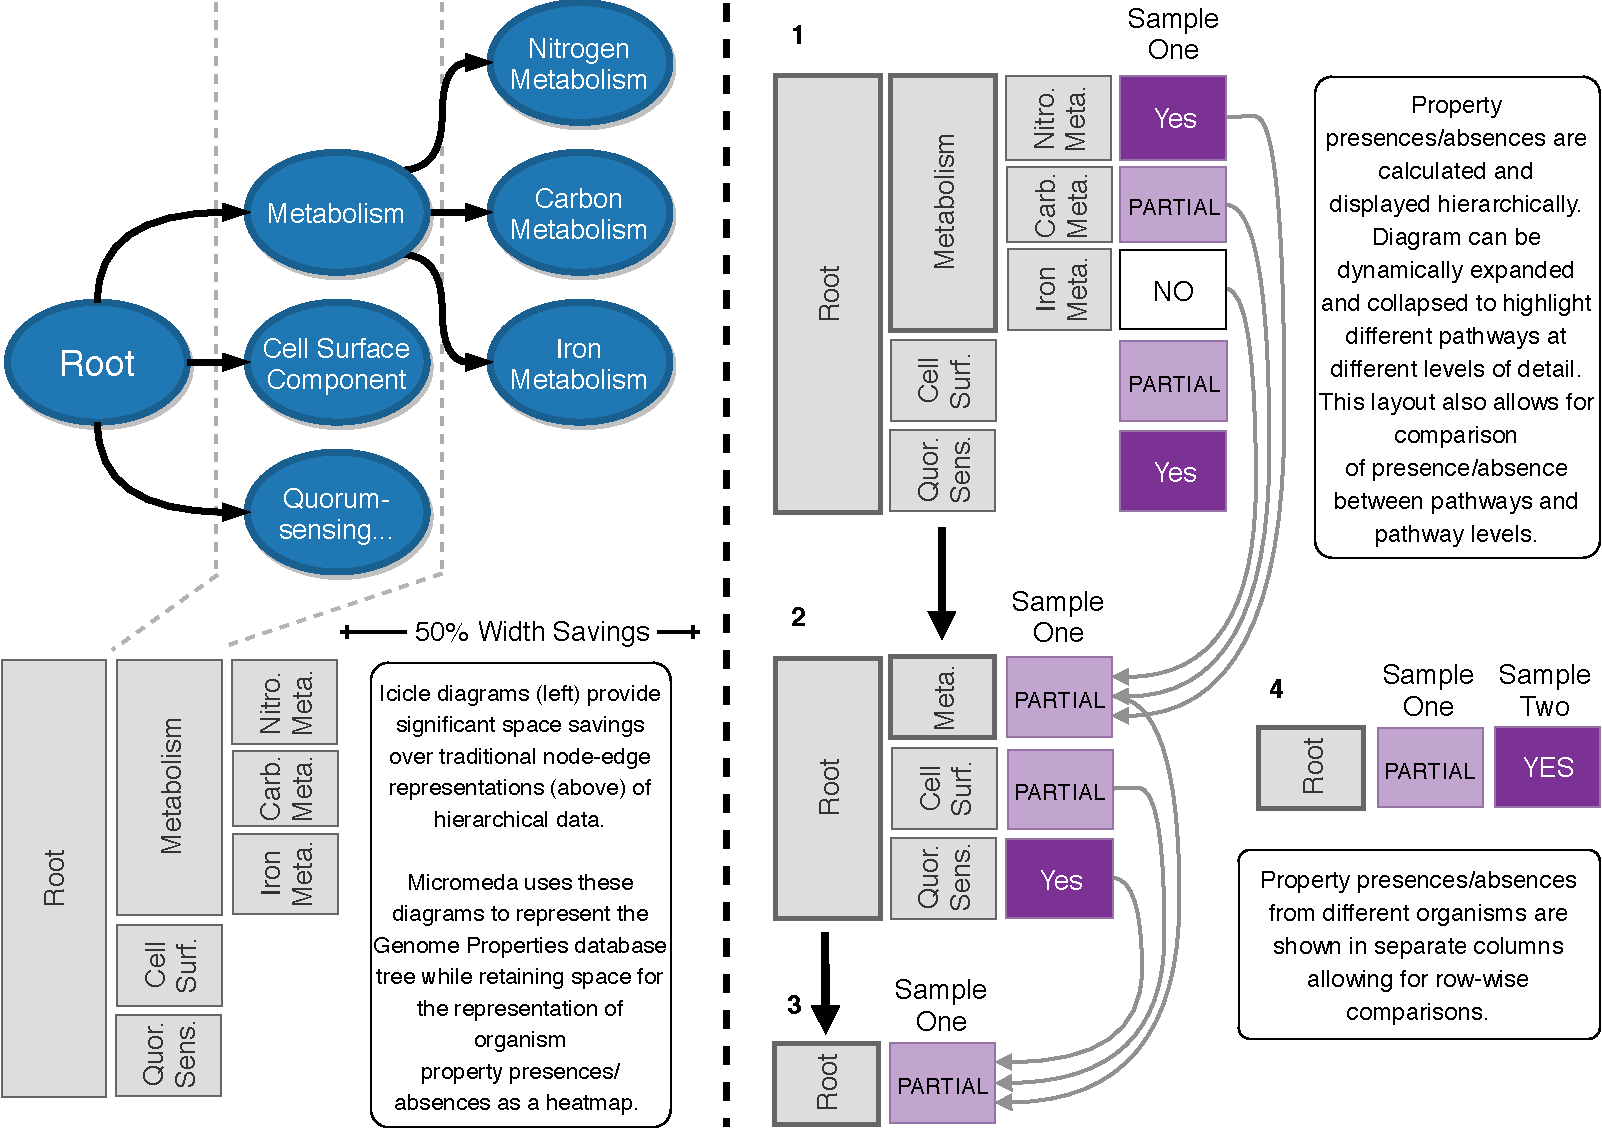
\includegraphics[width=\textwidth]{media/visualization_design_philosphy.pdf}
	 \caption{Micromeda-Client's user interface uses a clickable icicle diagram to change the state of an adjacent heat map of property and step assignments. Clicking nodes in the diagram changes the shape of the heat map by adding and removing rows from the diagram.}
	 \label{fig:visualization-philosophy}
\end{figure}

One key design decision for Micromeda-Client was how to let users control the above aggregation and de-aggregation of heat map rows. To support this usage, the author added a new visualisation component in addition to the assignment heat map. Specifically, Micromeda-Client uses a horizontal icicle diagram \footnote{Traditional icicle diagrams have leaf nodes facing downwards. The icicle diagram used by Micromeda-Client is rotated 90 degrees and has it leaf nodes facing to the right.} placed left of the heat map. This icicle diagram is used to control the heat map's content (Fig. \ref{fig:visualization-philosophy}). Icicle diagrams allow for the display of hierarchical data such as the relationship between properties and between properties and steps. Nodes which represent properties are labelled gray and those representing steps are labelled green. In Micromeda-Client, each of the genome properties and steps in the Genome Properties database is assigned a node in the icicle diagram (Fig. \ref{fig:visualization-philosophy}). The leafs of this icicle diagram are aligned to matching rows in the adjacent heat map (Fig. \ref{fig:visualization-philosophy}). Icicle diagrams were chosen over other ways of visualizing hierarchical data, such as trees, due to their spacial compactness (Fig. \ref{fig:visualization-philosophy}). With Micromeda-Client, the nodes in the icicle diagram are given a state of either on or off. When a node in an off state is clicked, a new column is added to the icicle diagram. This column's contents includes nodes representing the clicked node's children. Simultaneously as the new child columns is added, matching assignment rows belonging to properties or steps that the child nodes represent are added and replace the clicked node's assignment row in the heat map. The clicked node's shape is expanded vertically to align with the top and bottom of its first and last child node cell, respectively. If the clicked node is clicked once again then the process above is reversed, child nodes and their assignment rows are removed from the visualization (Fig. \ref{fig:visualization-philosophy}), the clicked cell returns to its original shape, and its matching summary assignment row is placed back into the heat map (Fig. \ref{fig:visualization-philosophy}). Columns in the icicle diagram are deleted, upon child cell removal, only if all sibling or cousin nodes to the clicked node have no children displayed.

The visualization strategy chosen for Micromeda-client supports the required tasks presented at the top of this section. The heat map allows users to track assignments across organisms and assess their magnitude. The interactive aggregation control provided by the icicle diagram allows for the aggregation of step and property assignments into summaries. These aggregate assignments can be de-aggregated to show child assignments, allowing users to explore how the parent assignment was derived. As the icicle diagram follows the structured of the Genome Properties DAG, specific assignments can be quickly found by following the DAG's structure from parent to child. Searching for properties is further enhanced by Micromeda-Client's ability to search for properties by name. This search functionality is discussed in the next section.

\section{Additional Features of Micromeda-Client's Interface}

In addition to the visualization capability presented above, the client's interface also possesses several other features which help users explore their data. In the top right corner of the user interface is a text-based search box (Fig. \ref{fig:micromeda-interface}). This allows user's to search for properties by name via entering a text string. As the user enters this string, matching property names are displayed in a drop down menu (Fig. \ref{fig:micromeda-interface}). If one of these property names is clicked, then the Micromeda-Client will automatically scrolls heat map to the row where assignments for the property are located. If the property is not shown in the current version of the heat map, then it will be added by expanding a path to the property. This paths is built via recursively de-aggregating parent properties along a path from the root of the Genome Properties DAG to the property which was clicked in the menu.

The scrolling behaviour above is also activated when a user clicks a node in the icicle diagram. When clicked, the heat map will scroll to align with the top of the clicked node. As the diagram scrolls the X-axis labels remain in a fixed position to provide users with context to which organisms assignments belong. 

\begin{figure}[!ht]
  \centering
	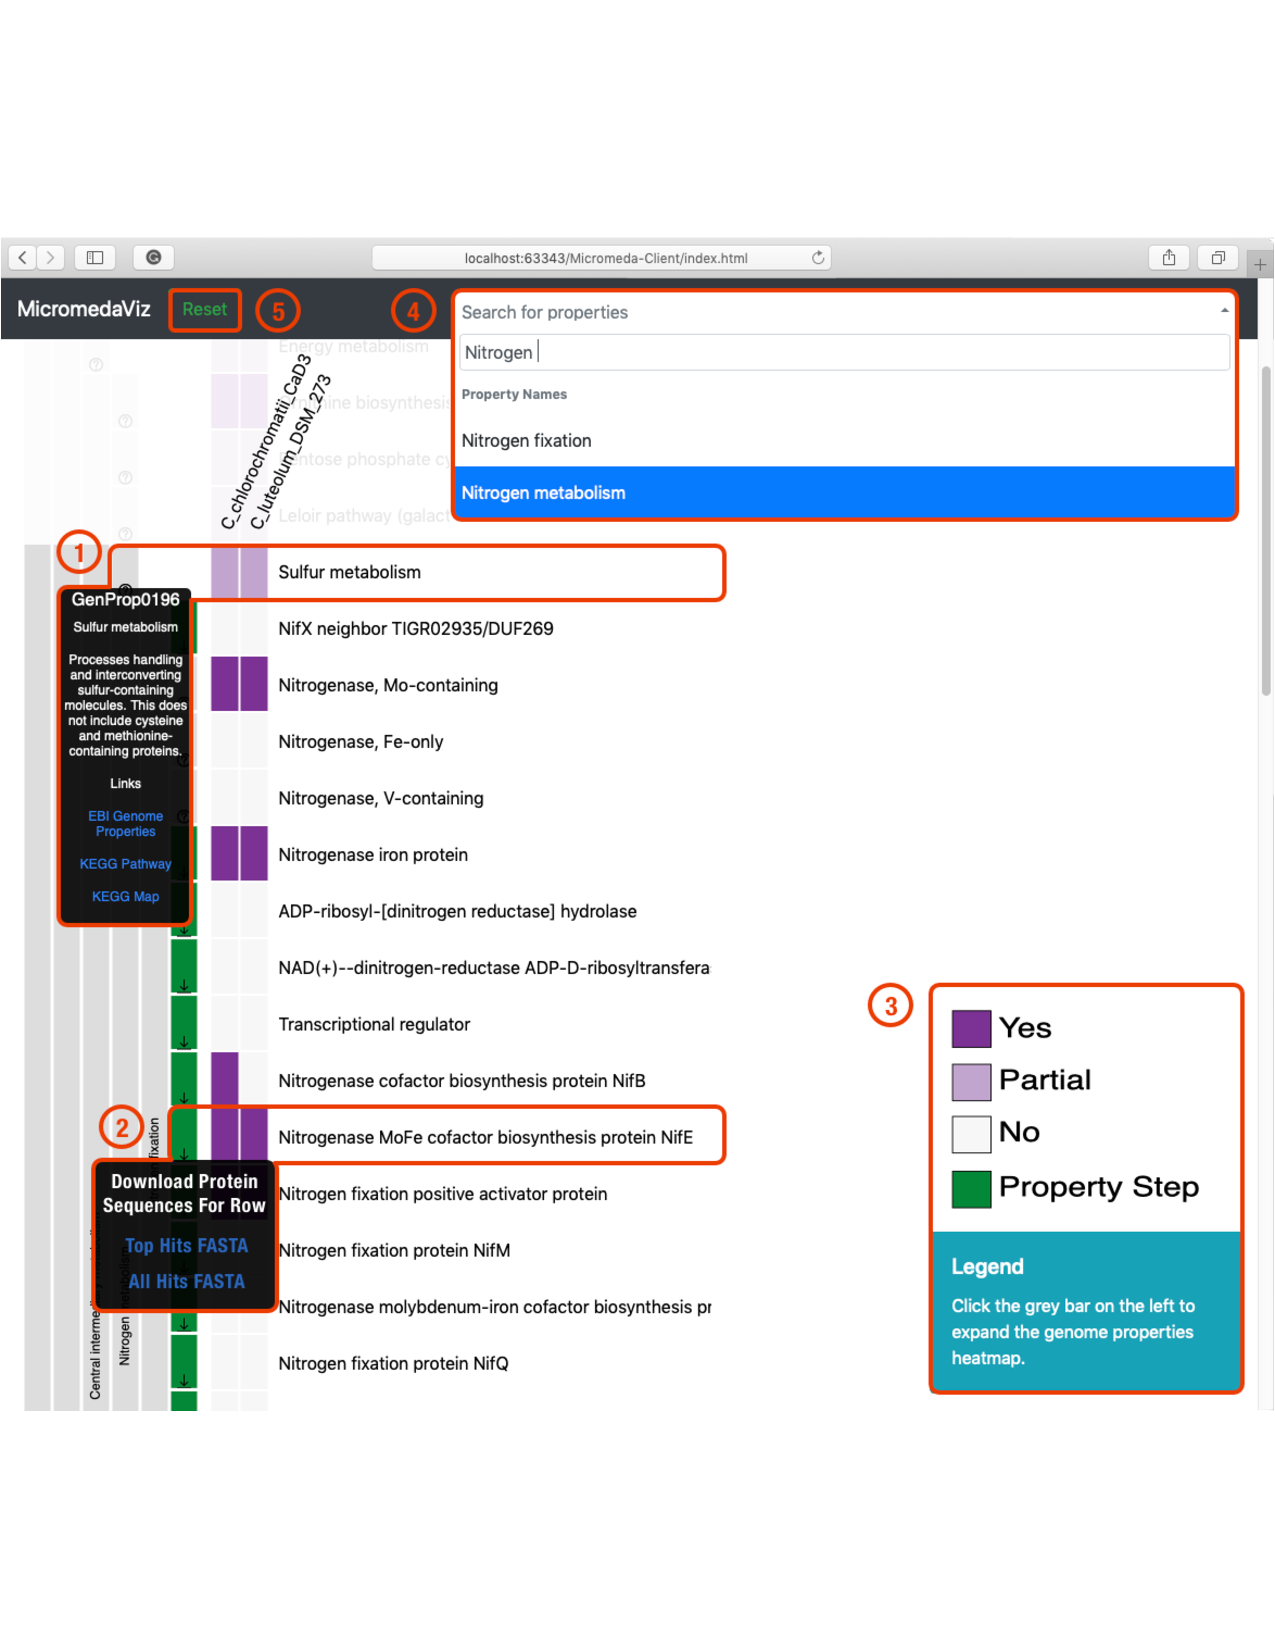
\includegraphics[width=0.9\textwidth]{media/micromeda-interface.pdf}
	 \caption{Micromeda's user interface provides functionality for searching for properties (4), getting additional information about properties and steps (1), and has the ability to download protein sequences which support step assignments (2). A legend provides context to the heat map's colours (3). A reset button allows users to reset the heat map to its initial load state(4).}
	 \label{fig:micromeda-interface}
\end{figure}

While users explore the genome property assignments of organism's in their datasets, it may be useful for them to be able to get more context about the properties whose assignments are displayed. To facilitate this, the icicle diagram has question mark glyphs at the bottom of each node. When these glyphs are hovered over, a pop up box appears displaying information about the property that the node represents (Fig. \ref{fig:micromeda-interface})). The pop up box includes the name of the property, a description of it, a link to the property in the EBI Genome Properties website, and a list of links to equivalent records in other pathways databases such as KEGG \cite{kanehisa2000kegg} and MetaCyc \cite{karp2002metacyc}. When the user's cursor leaves the glyph or the pop box, the box is once again hidden.

Property steps have a different glyph at the bottom of their nodes that look like a download symbol (Fig. \ref{fig:micromeda-interface})). It may be useful for users to be able to download protein sequences that support the existence of property steps across organisms in an uploaded dataset and the the pop up box of this glyph supports that. When the download glyph is hovered over, it opens up pop up box containing two download links (Fig. \ref{fig:micromeda-interface})). The first link, when clicked, downloads a FASTA file containing the protein sequences that are most likely to carry out the step in each organism in a dataset. The second link points towards a second FASTA file containing any protein that could carry out the step in a dataset. When the cursor is removed from this download pop up box, it will be hidden

Micromeda-Client's interface also includes a reset button. This button resets the heat map and icicle diagram back to their original configuration where only top level properties are shown (i.e., one level below the root in the Genome Properties DAG). Its is useful for when users want to reset the diagram to search for other properties.

\section{Delivery Methodology}

Micromeda-Client is delivered as a client web browser application. The method was chosen due to its relative ease of deployment. End users only need open the web address of the client for the client to be loaded into their web browser and run. Since the application is web browser-based, it will work on any operating systems with a modern web browser and even mobile devices such as tablet computers and cell phones.

\section{Implementation}

Micromeda-Client's interface consists of two web pages that were structured using Hypertext Markup Language 5 (HTML5) \cite{HTML5}, styled using Cascading Style Sheets 3 (CSS3) \cite{CSS3}, and scripted via JavaScript (ECMAScript 6) \cite{flanagan2006javascript}. One page is used for uploading user generated Micromeda files and another is used for presenting the visualizations of the file's data to users. To use Micromeda-Client, users must first navigate to the upload page and upload a Micromeda file. After upload is complete, their browse will automatically redirect them to the visualisation page. Both pages are styled using the Bootstrap 3.0 CSS framework \cite{spurlock2013bootstrap}. Bootstrap is used set up page elements such as header navigation bars and drop down menus. Bootstrap also makes each of the pages compatible with tablet computers and phones as it will automatically restyle the pages to fit on these device's smaller screens.

\subsection{Core Data Structures} \label{visual-data-structures}

Two core data structures are used by the client visualization page and they are both used during diagram generation. One is a diagram configuration array which contains a series of measurements which are used during diagram drawing. These measurements control things such as the spacing between heat map cells, heat map cell dimensions and the offset of axis labels. A summary of these measurements can be seen in Fig. \ref{fig:diagram-measurements}. The contents of this setting array is stored in a JSON file \cite{bray2014rfc}, called \textbf{diagram\_configuration.json}, which is deployed alongside the HTML files of the client. The second data structure is a copy of the Genome Properties DAG in the form a tree (i.e., nodes with two parents are duplicated) of JavaScript objects. Each of these objects represents a genome property or step and objects are linked together in parent-child relationships. This data structure is analogous to the one used by Pygenprop (Section \ref{GenomePropertiesTree-Class}).  Each of these objects possesses an attribute, called assignments, containing a list of property assignments for a set of organisms. The objects also have an attribute, called \textbf{enabled}, containing a boolean (i.e., true or false). The contents of the visualization presented by the client  maps directly to the state of property object tree (Fig. \ref{fig:tree-map-to-viz}). When the property tree manipulated by the client and the clients visualization is redrawn, it is redrawn in a way that matches the new structure of the tree. The \textbf{enabled} boolean of each property object tree provides determines whether the children of the property should be displayed in the client's assignment heat map and icicle diagram (Fig. \ref{fig:tree-map-to-viz}). Elements of Micromeda's user interface manipulate enabled states of objects in the property tree and this in turn can manipulate the contents of the visualization (Fig. \ref{fig:tree-map-to-viz}). The property tree is placed within a parent JavaScript object. This object also possesses methods for dictionary style look ups of properties from the tree based on their property identifier and selection root and leaf properties, which is analogous to Pygenprop's GenomePropertiesTree class (Section \ref{GenomePropertiesTree-Class}).

\begin{figure}[!ht]
  \centering
	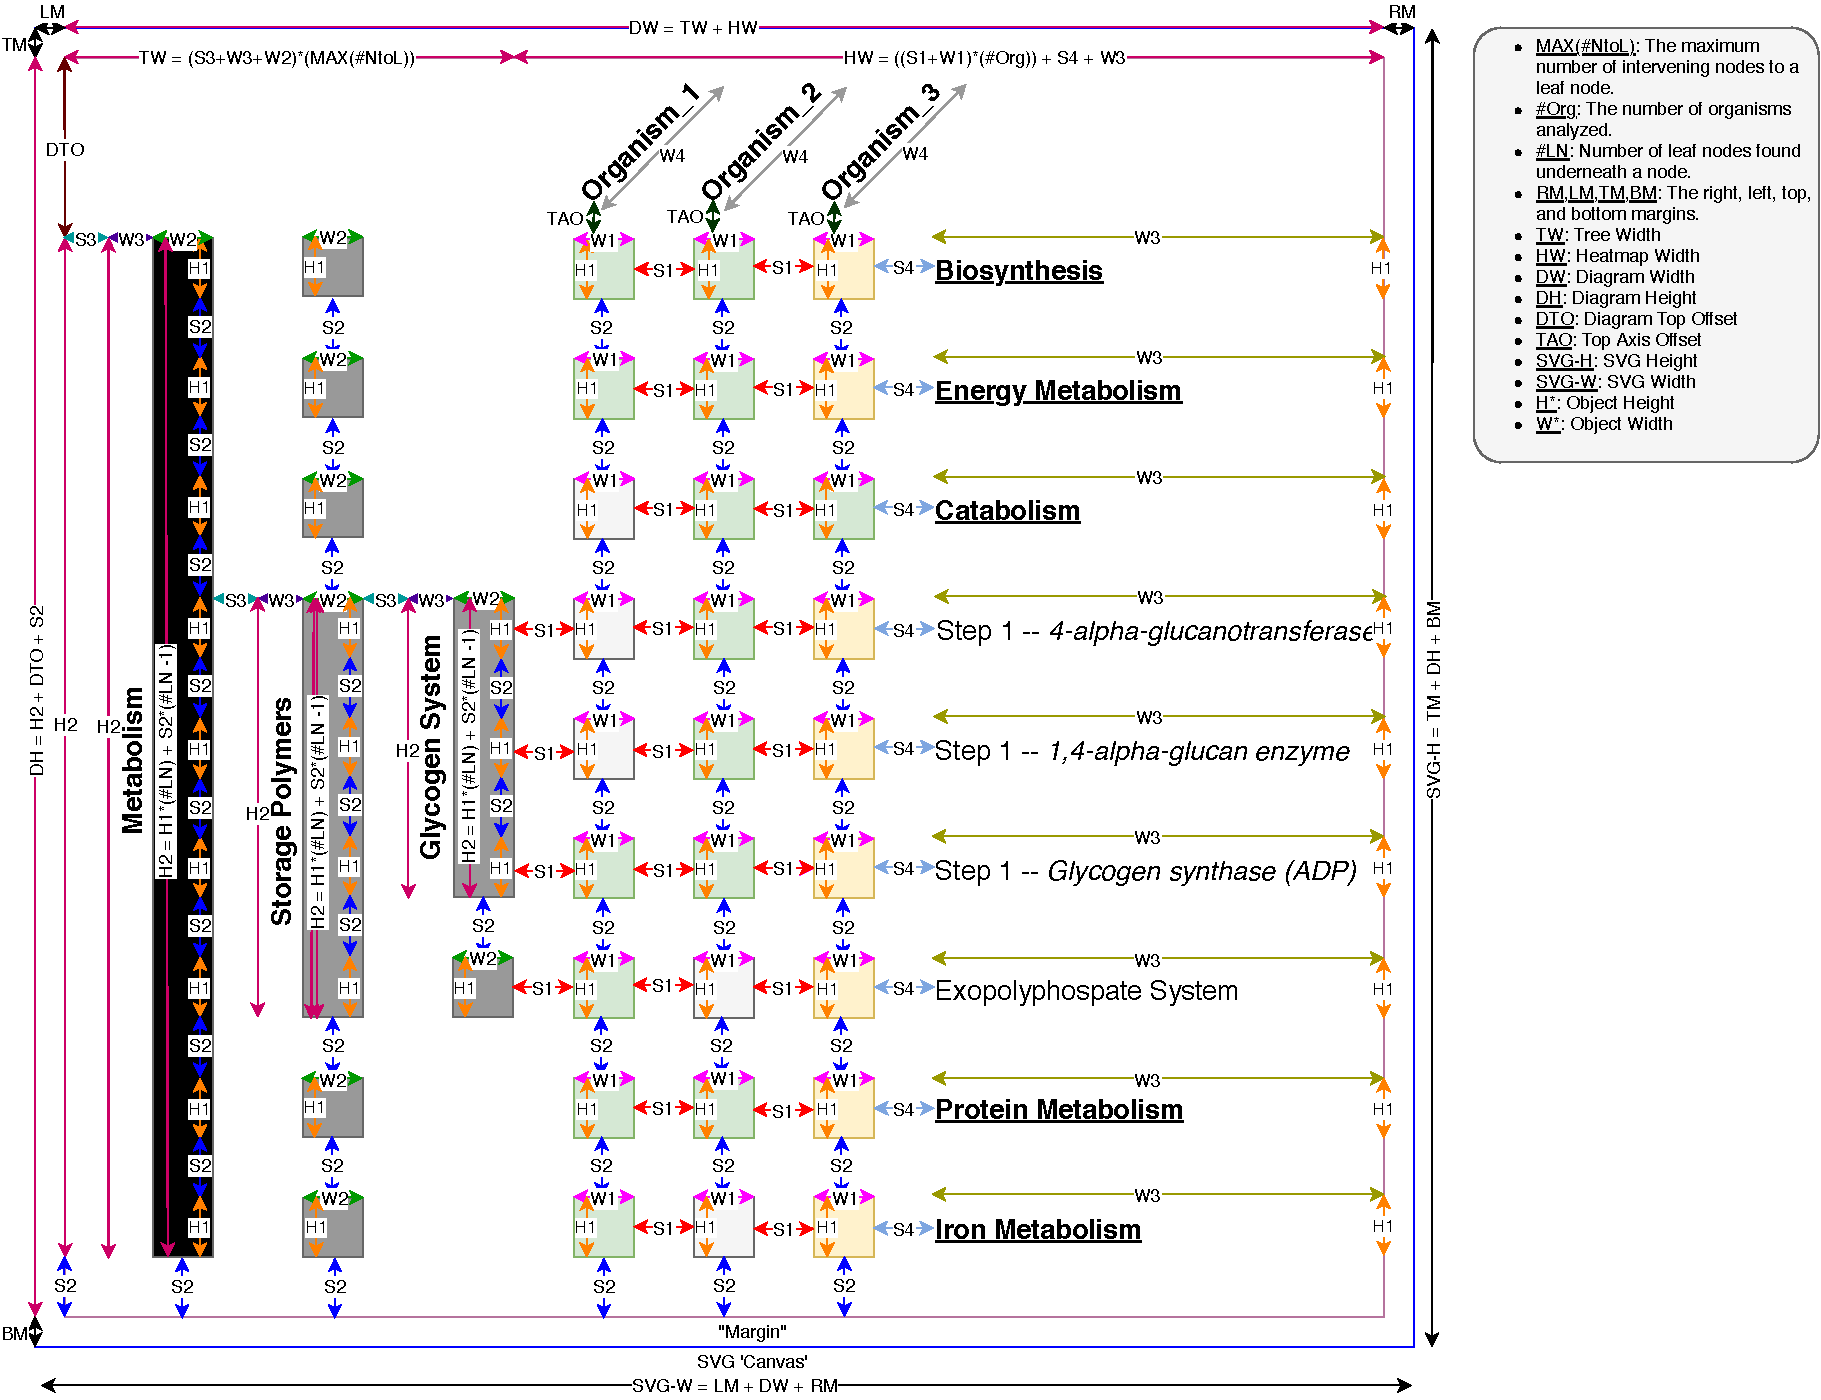
\includegraphics[width=\textwidth]{media/diagram_measurements.pdf}
	 \caption{A series of spacing, width and length values are used by Micromeda-Server to build its diagrams. These values are stored in an external file. The contents of this file can be modified to change the the layout of Micromeda-Client's visualizations.}
	 \label{fig:diagram-measurements}
\end{figure}

\begin{figure}[!ht]
  \centering
	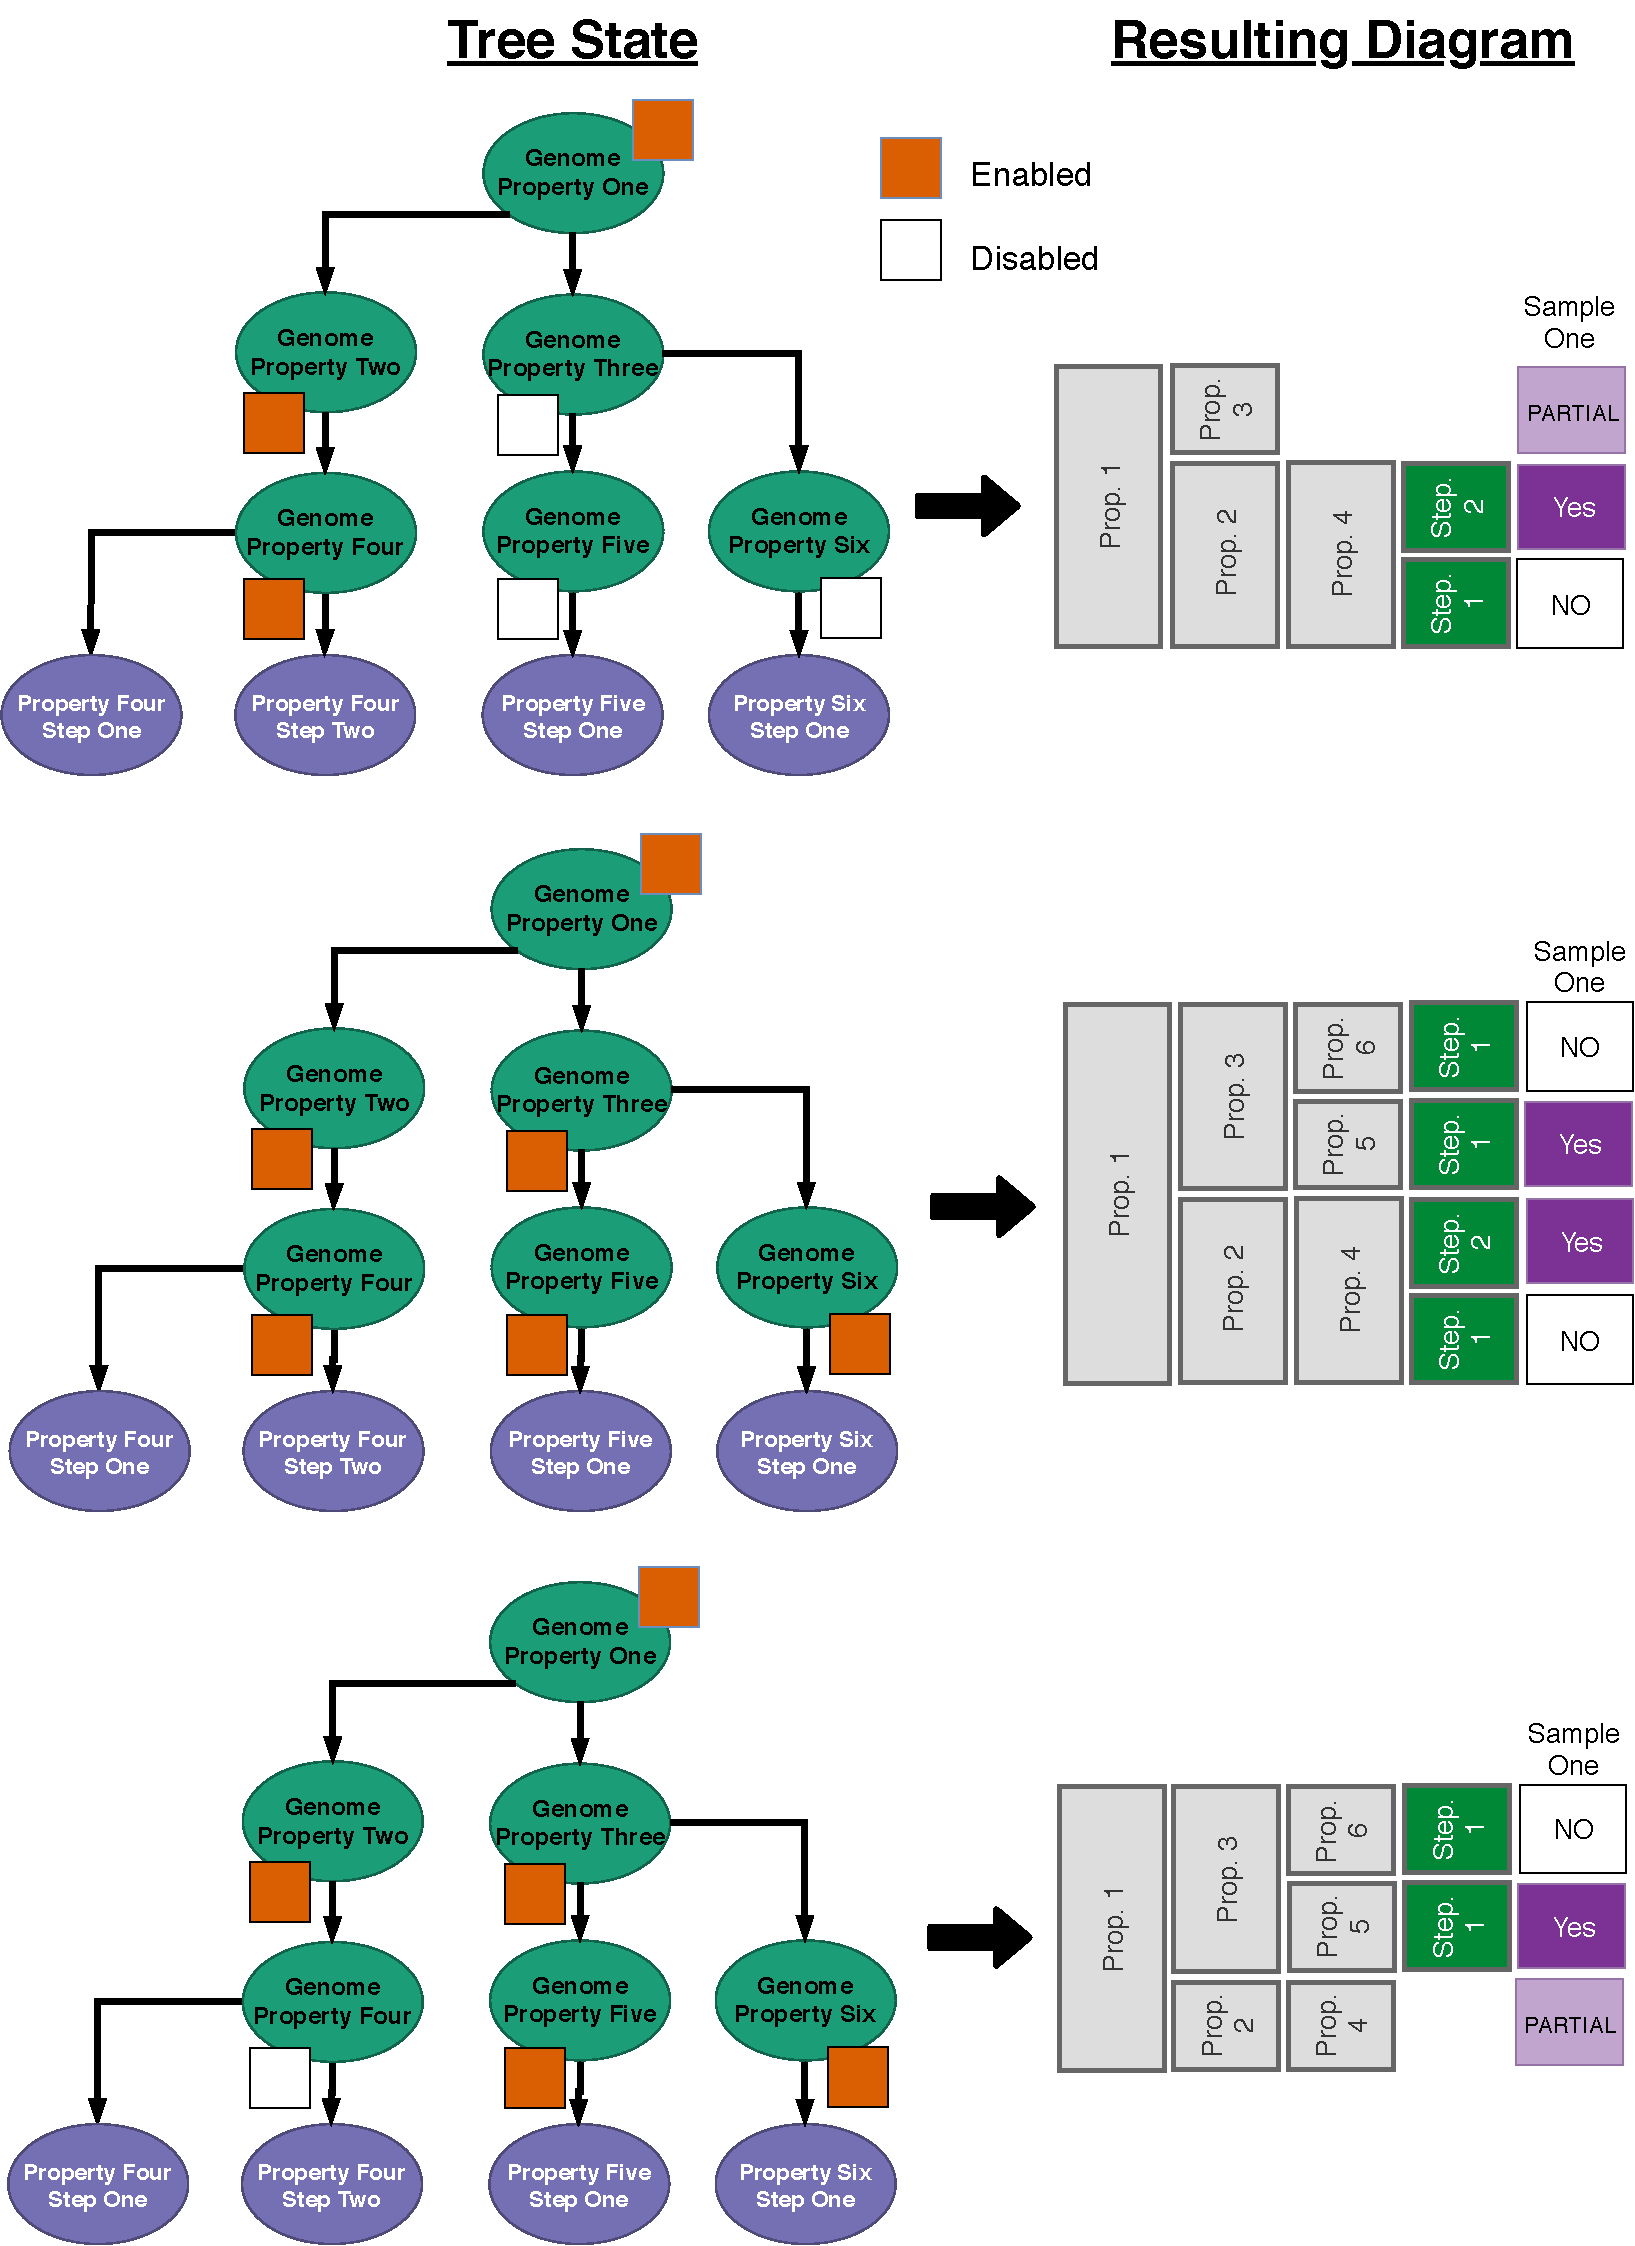
\includegraphics[width=0.7\textwidth]{media/how_tree_state_maps.pdf}
	 \caption{The state of enabled attributes in the client's Genome Property tree directly maps to contents of its visualization.}
	 \label{fig:tree-map-to-viz}
\end{figure}

\subsection{Loading the Visualization}

As mentioned previously, much of the functionality of Micromeda-Client is supported by requests for data from Micromeda-Server. All these requests are done through a technique known as Asynchronous JavaScript and XML (AJAX) \cite{garrett2005ajax,li2012jquery} (see \href{en.wikipedia.org/wiki/Ajax\_(programming)}{en.wikipedia.org/wiki/ Ajax\_(programming)}). AJAX allows requests to be made to the server, using JavaScript \cite{flanagan2006javascript}, without the need for a web page reload. This technique allows Micromeda-Client to remain asynchronous and not kept in sync with the server to where it was downloaded. AJAX requests are made via Hypertext Transfer Protocol (HTTP) \cite{fielding1999hypertext}, through a series of Uniform Resource Locator (URL) addresses \cite{berners1994rfc} which map to Micromeda-Server endpoints (Section \ref{endpoints}). All AJAX requests to the server were made using the JQuery JavaScript library \cite{chaffer2013learning,li2012jquery}. The URL address of Micromeda-Server, where AJAX requests are made to, is found in a JSON file called server\_config.json, which is deployed with HTML files of the client. This file is loaded by both the file upload and visualization page upon their initial load.

The upload page contains a file drag and drop zone and when a user drops a Micromeda file on this zone it is sent, via AJAX, to Micromeda-Server using its \textbf{upload} endpoint (Subsection \ref{endpoint-upload}). The drag and drop zone was implemented using DropzoneJS \cite{meno}. After the file upload is complete, a dataset key is returned to Micromeda-Client. This dataset key is stored in the browser's web local storage \cite{Hickson} (\href{en.wikipedia.org/wiki/Web\_storage}{en.wikipedia.org/wiki/Web\_storage}) using a library called localForage \cite{localforage} \footnote{LocalForage (\href{github.com/localForage/localForage}{github.com/localForage/localForage}) is a wrapper library for a variety of web browsers' local storage systems. It provides Micromeda-Client with compatibility with broad range of browsers including those with more outdated local storage systems such as the one possessed by older versions of Safari \cite{lawson_2014}.} Once the dataset key is stored, the browser is redirected to the visualisation page where the visualization of uploaded file's contents is generated.

As the visualisation page loads, the client requests a JSON tree from Micromeda-Server's \textbf{get\_tree} endpoint (Subsection \ref{get-tree}) via AJAX. The dataset key saved in local storage is provided with this request and ensures that data from the recently uploaded Micromeda file is returned. Micromeda-Server will respond to the request to the \textbf{get\_tree} endpoint by returning JSON tree containing assignments for all properties and steps within the uploaded Micromeda file. This JSON file is parsed into a JavaScript tree, which is used as the core property tree data structure mentioned in Section \ref{visual-data-structures} above. The visualization is then built using the dimensions from the diagram configuration array, the contents of the property tree and the \textbf{enabled} attribute of the property objects therein. The visualisation are generated using version 3.0 of the D3.js visualization library \cite{bostock2015d3} and custom JavaScript library.

\subsection{Interactivity After Initial Visualization Load}

One of the key properties of clients visualizations is that it is interactive and this interactivity is provided by manipulating the JavaScript property tree. When a property node in the icicle diagram is clicked, an JavaScript DOM (Document Object Model) onclick event \cite{dom-events} (\href{en.wikipedia.org/wiki/DOM\_events}{en.wikipedia.org/wiki/DOM\_events}) is triggered, which changes that  state of equivalent property object in the core property tree data structure. Specifically, the clicked node's equivalent property object's \textbf{enabled} attribute is inverted upon icicle node click (Fig. \ref{fig:tree-map-to-viz}) and the entire visualisation is subsequently re-rendered. Because the enable attribute has changed on the property object, the heat map visualization is re-rendered in a different configuration (Fig. \ref{fig:tree-map-to-viz}). 

In the case where a leaf node on the icicle diagram is clicked, the matching property object's \textbf{enabled} attribute is changed from false to true. Then when the diagram is subsequently re-rendered, the children of the clicked node are now rendered (Fig. \ref{fig:tree-map-to-viz}). After this re-rendering, the page is scrolled so that the bottom of the X-axis labels are aligned with the top of the clicked node. The opposite occurs when a non-leaf node on the icicle diagram is clicked. The associated property object's \textbf{enabled} variable is changed from true to false and after re-rendering of this node's children are removed. The page is scrolled so the bottom of the X-axis labels are aligned with the top of the clicked node. The true and false state of child property objects is not changed. This provides the visualization with a sort of "memory". When a child node is re-enabled on the diagram the state of its children is retained (Fig. \ref{fig:tree-map-to-viz}).

At page load the property tree is used to create an JavaScript array of pairs of property names and identifiers. After the visualisation generation, an interactive search menu is created in the top right hand corner of the Micromeda-Client interface (Fig. \ref{fig:micromeda-interface})). This menu is built using the Select2 library \cite{select2} (\href{select2.org}{select2.org}) and uses previously mention pairs of property identifiers and names as search data. When a property name or identifier is searched for in the search menu, properties whose name is similar to the search query are displayed in a drop down menu (Fig. \ref{fig:micromeda-interface})).

When one of these menu properties are clicked then another JavaScript event occurs where the parent of the matching property object in the JavaScript property tree is modified. All property objects along the tree in a path from the root to the parent of matching property object have their \textbf{enabled} attribute set to true. Thereafter, when client visualization is subsequently re-rendered, a path to the assignments of the clicked property is displayed along with the property's assignments. The page is scrolled so the bottom of the X-axis labels are aligned with the top of the clicked node.

After each re-rendering of the assignment visualization, a series of AJAX requests sent. These are requests for information about each property that is visible in the icicle diagram (Fig. \ref{fig:micromeda-interface})). These requests are sent to Micromeda-Server's \textbf{Get\_Single\_Genome\_Property \_Info} endpoint (Subsection \ref{get-property-info-endpoint}). The endpoint returns a JSON document containing the information about a property, which is later used in property information pop up boxes (Fig. \ref{fig:micromeda-interface})). The contents of these documents are also cached in web local storage using localForage \cite{localforage}. During subsequent diagram re-renderings requests are not made for properties whose data is already cached. This caching reduces request frequency to the server and overall server load. The request volume is also reduced by only making requests  for properties that are visible.

Both property information and FASTA download pop up boxes are generated upon activation of JavaScript onmouseover events \cite{dom-events} (\href{en.wikipedia.org/wiki/DOM\_events}{en.wikipedia.org/wiki/DOM\_events}) of the property question mark and step download glyphs, respectively. When the a question mark glyph of a property icicle diagram node is hovered over, information about the property is retrieved from the web local storage using localForage. This property information was cached during the last time the diagram was rendered, and a template of this information is used if no information for a specific property is found. The property information is used to generate the contents of property information pop up box. The FASTA download pop box, when generated contains links for downloading FASTA files. These links point to URLs provided by Micromeda-Server's \textbf{get\_fasta} endpoint (Subsection \ref{get-fasta-endpoint}). When the get all proteins link is clicked (Fig. \ref{fig:micromeda-interface})), the endpoint URL's \textbf{all} HTTP GET parameter is set to true during the request and thus FASTA file containing all proteins that support the step is downloaded (see Subsection \ref{get-fasta-endpoint}). The \textbf{all} HTTP GET parameter is not added during requests initiated by clicking the get top proteins link. The lack of this parameter leads to the downloaded  FASTA file containing only the proteins that are most likely to support a step. During both of these requests, both for all and only the top proteins, the dataset key stored in web local storage is provided. This key tells the Micromeda-Server to generate FASTA files from protein sequences stored in the recently uploaded Micromeda file. Both pop boxes are hidden upon removal of the users cursor. This hiding functionality is triggered by a onmouseout event \cite{dom-events} (\href{en.wikipedia.org/wiki/DOM\_events}{en.wikipedia.org/wiki/DOM\_events}).

\section{Interface Performance}

It was found that, other then those that wait for data from Micromeda-Server, all interactive components of Micormeda-Client had almost no visual lag attributed to their construction. For example the visualisation was capable of being re-rendered almost instantaneously even when several hundred rows of assignments were to be displayed.

\section{End-User Testing}

Three potential user of Micromeda-Client were provide with visualization of data relevant to their research project. These users were interviewed afterwards and their suggestions for improving the clients user interface recorded. Some of their suggestions are discussed in Section \ref{client-improvements}. 

\section{Deployment}

Micromeda's user interface can be deployed in two ways. It can be served from a web server, such as NGINX \cite{reese2008nginx}, running on the same server computer system as Micromeda-Server (Fig. \ref{fig:client-deployment}). Such a web server is already of component of the medium scale deployment of Micromeda-Server described in Subsection \ref{single-server-micromeda-deployment}. It can also be served from a Content Delivery Network (CDN) \cite{farber2003internet} (\href{en.wikipedia.org/wiki/Content\_delivery\_network}{en.wikipedia.org/wiki/Content\_delivery\_network}) such as Amazon Cloudfront \cite{varia2014overview} (\href{aws.amazon.com/cloudfront}{aws.amazon.com/cloudfront}) or Cloudflare Anycast \cite{calder2015analyzing} (\href{cloudflare.com/cdn}{cloudflare.com/cdn}). In this deployment configuration, the end user downloads the client code from nearest content delivery server in the the CDN, rather than the same sever as to where Micromeda-Server is hosted (Fig. \ref{fig:client-deployment}). After loading, the client would then still send API requests to Micromeda-Server, which would be hosted outside the CDN (Fig. \ref{fig:client-deployment}). For development purposes the files for Micromeda-Client could also be downloaded and opened by a developer's web browser for testing purposes.

\begin{figure}[!ht]
  \centering
	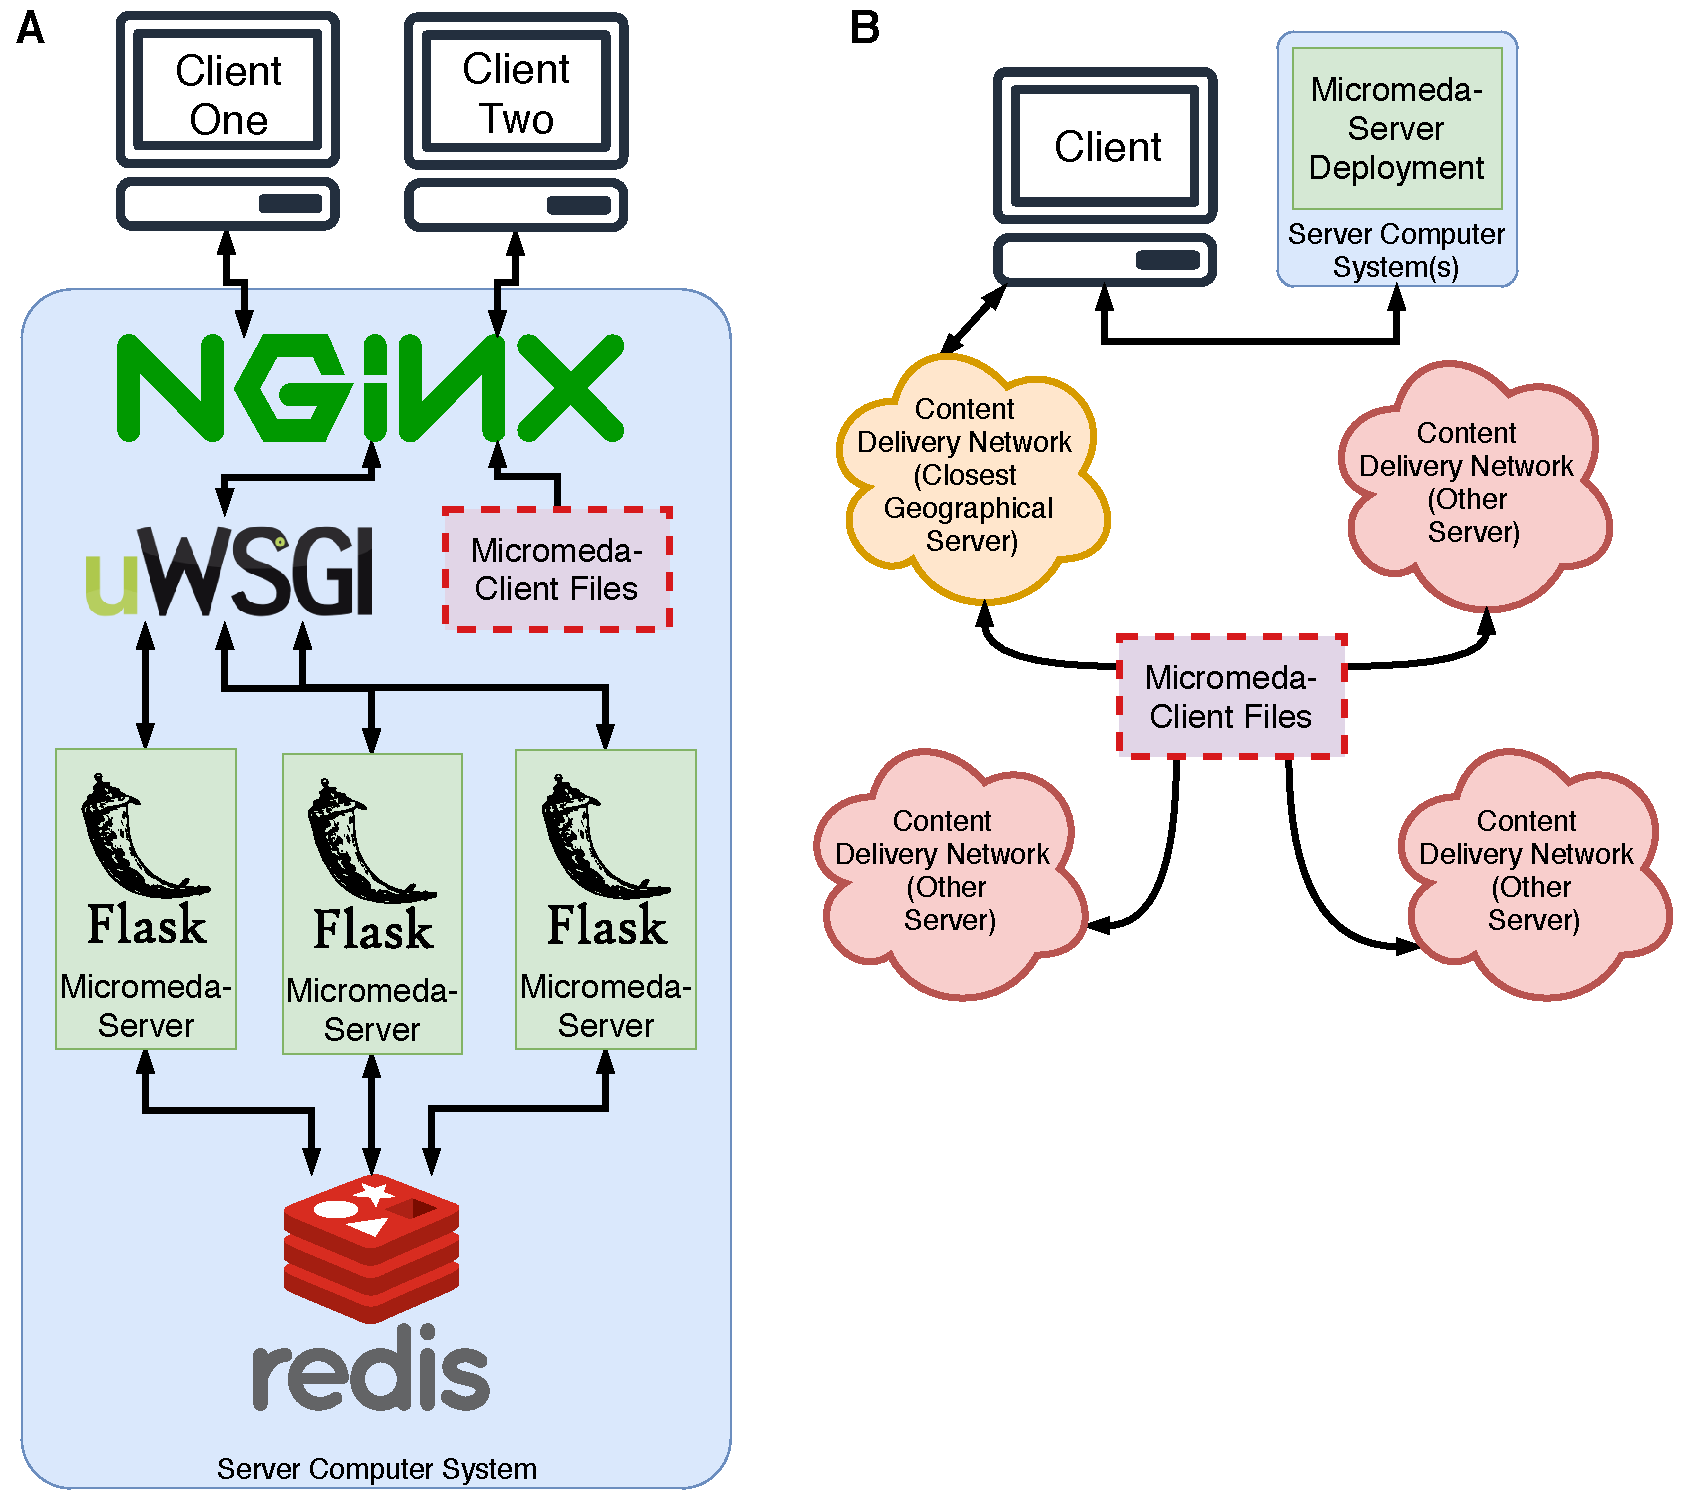
\includegraphics[width=0.7\textwidth]{media/micromeda-client-deployment.pdf}
	 \caption{The client files for Micromeda-Client, in production, can either be deployed on the same server computer system as Micromeda-Server (A) or via a content delivery network (B).}
	 \label{fig:client-deployment}
\end{figure}

\section{Future Improvements} \label{client-improvements}

\section{Summary} 